\documentclass[11pt,a4paper]{article}
\usepackage[utf8]{inputenc}
\usepackage{amsmath}
\usepackage{amsfonts}
\usepackage{amssymb}
\usepackage{makeidx}
\usepackage{graphicx}
\usepackage[width=15.00cm, height=23.00cm]{geometry}
\usepackage{enumerate}
\usepackage{titlesec}
\usepackage[spanish]{babel}
\usepackage{fancyhdr}
\usepackage[usenames]{color}
\setlength\parindent{0pt}

\titleformat{\paragraph}
{\normalfont\normalsize\bfseries}{\theparagraph}{1em}{}
\titlespacing*{\paragraph}
{0pt}{3.25ex plus 1ex minus .2ex}{1.5ex plus .2ex}

\renewcommand{\headrulewidth}{0pt}

\rhead{Especificación de Requisitos Software VIRUTA \\ \today
}
\lhead{}

\pagestyle{fancy}

\begin{document}


\begin{titlepage}
\vspace*{8cm}
\begin{center}
{\Huge \textsf{Especificación de \\ requisitos software \\ VIRUTA}}\\

\vspace*{2cm}

\textsf{\Large \today}
\end{center}
\end{titlepage}

\tableofcontents
\thispagestyle{empty}
\newpage


\section{Introducción}

\subsection{Propósito}

El objetivo de la especificación de requisitos software (ERS) es describir de forma concisa los servicios y restricciones de nuestro sistema software. La ERS establece una base de acuerdo o contrato entre la empresa de transporte TRASNFER y la empresa proveedora del servicio informático, APPCOM. Este documento proporciona una guía de la estructura y funcionalidad del sistema.\\

Nótese que este documento no contendrá referencia alguna a detalles concretos sobre la implementación de dicho software informático.

\subsection{Ámbito}

El sistema informático a desarrollar, al que de ahora en adelante llamaremos VIRUTA, tendrá como propósito la venta automatizada de billetes de tren en la red de Cercanías. VIRUTA permitirá al personal revisor de TRANSFER efectuar la venta e impresión de billetes no numerados directamente en el tren, ahorrando al viajero la necesidad de pasar por la taquilla.\\

Dicha venta de billetes será sujeto de aplicación de los distintos descuentos y tarifas que TRANSFER considere oportunos.\\

VIRUTA deberá interactuar con el servidor central de TRANSFER para actualizar rutas, horarios, tarifas y descuentos, y para descargar todas las operaciones realizadas, que habrán quedado asociadas al empleado de TRANSFER que las llevó a cabo.\\

Por el contrario, VIRUTA no tendrá capacidad de conexión inalámbrica, por lo que por ejemplo, no aceptará pagos con tarjeta (estos serán exclusivamente en efectivo), ni dispondrá de actualizaciones automáticas del sistema.\\

\color{red} VIRUTA correrá en terminales de punto de venta modelo MOTOROLA XLS 6000 que serán propiedad de TRANSFER. En un plazo de no menos de 2 años, dichos terminales habrán sido progresivamente remplazados por el modelo superior XLS 9000. Dichos terminales podrán ser usados indistintamente por cualquier empleado de TRANSFER que sea responsable de llevar a cabo las ventas. \color{black} \\


Por último, VIRUTA no deberá ser capaz de tramitar multas a los pasajeros, quedando esta funcionalidad restringida a los procedimientos actuales definidos por TRANSFER para la misma.
VIRUTA supondrá evidentes ventajas y ahorro de costes tanto para TRANSFER como para sus clientes.\\

\begin{enumerate}
\item Permitirá a TRANSFER reducir los recursos destinados a venta en taquilla. Por ejemplo, ya no será necesario disponer de personal de taquilla en aquellas localidades con escaso tránsito de pasajeros.
\item Permitirá a TRANSFER un seguimiento automatizado de los volúmenes de ventas y pasajeros.
\item Permitirá a los clientes de TRANSFER un ahorro en tiempo y una ganancia en comodidad al poder pagar sus trayectos directamente en el tren.
\end{enumerate}

\subsection{Definiciones, acrónimos y abreviaturas}

\begin{itemize}
\item ERS: Especificación de requisitos software, el presente documento.
\item TRANSFER: Transportes Ferroviarios. Empresa encargada de la explotación de los trenes de cercanías.
\item VIRUTA: Venta de billetes en ruta. La aplicación a desarrollar mediante la presente ERS.
\item Revisor: Personal de TRANSFER encargado de la venta y comprobación de los billetes en las rutas explotadas por TRANSFER.
\item Trayecto: Viaje entre dos nodos de la red de TRANSFER.
\item Billete: Documento que certifica el derecho de un cliente a realizar un trayecto en la red de TRANSFER. Viene definido por dicho trayecto, la fecha y hora, y la tarifa y descuento aplicados al mismo.
\item Tarifa: Precio asignado por TRANSFER a un trayecto.
\item SC: Sistema Central informático de TRANSFER
\item TPV: Terminal de punto de venta.
\item V-Ops: VIRUTA operaciones. Nombre del formato usado para transmitir las operaciones realizadas a lo largo del día del TPV al SC.
\item V-Trf: VIRUTA tarifas. Nombre del formato usado para transmitir la información de tarifas del SC al TPV.
\item V-Usr: VIRUTA usuarios. Nombre del formato usado para transmitir la información de usuarios del SC al TPV.
\item V-Dsc: VIRUTA descuentos. Nombre del formato usado para transmitir la información de descuentos del SC al TPV.

\end{itemize}

\subsection{Referencias}
Como referencia se ha usado la siguiente página la guía del Std. 830 del IEEE para la especificación de requisitos Software, así como los apuntes del tema 10 del Máster de Gestión y Dirección de Proyectos Software.


\subsection{Visión global} 

El resto de la ERS está organizada siguiendo el siguiente esquema:\\


{\Large Descripción general:} describe los factores generales que afectan al producto y sus requisitos.
\begin{itemize}
\item Perspectiva del producto: establece el contexto de implantación del producto y el uso del interfaz del sistema, interfaces de usuario, hardware, interfaces de comunicación, etc.
\item Funciones del producto: describe las funciones principales del software.
\item Características de usuario: describe el nivel educativo, experiencia y capacidad del usuario.
\item Restricciones: Políticas de regulación, limitaciones hardware e interfaces con otras aplicaciones, operaciones en paralelo, funciones de auditoria y de control, requisitos de fiabilidad, etc.
\item Supuestos y dependencias: Identifica los factores que afectan a los requisitos de la SRS.
\item Requisitos futuros: indicará los requisitos que se incluirán en versiones futuras del software.
\end{itemize}

{\Large Requisitos específicos:} Contienen todos los requisitos del sistema, con nivel de detalle mayor que el apartado anterior. Constituye la base del diseño que posteriormente será implementado.
\begin{itemize}
\item Interfaces: descripción detallada de todas las entradas y salidas del sistema software.
\item Funciones: define las acciones fundamentales que tendrán lugar en el software durante la aceptación y procesamiento de la entrada y durante el procesamiento y generación de la salida.
\item Requisitos de Rendimiento: requisitos numéricos estáticos y dinámicos del rendimiento del sistema.
\item Requisitos de la Base de datos lógica: Requisitos lógicos de la información que residirá en la base de datos.
\item Restricciones de Diseño: Restricciones impuestas al diseño por adecuación a otros estándares, limitaciones hardware, etc.
\item Atributos del sistema software: Características del sistema software no funcionales. Aquí se evalúan conceptos como fiabilidad, robustez, velocidad, etc.
\end{itemize}

\section{Descripción general}

\subsection{Perspectiva del producto}

\color{red}

VIRUTA debe ser implantado en un entorno de explotación específico y dependiente de otros sistemas ya existentes. Como ya se ha enunciado anteriormente, la aplicación deberá correr en terminales MOTOROLA XLS 6000 que se irán remplazando progresivamente por el modelo superior XLS 9000 dentro de un plazo de dos años.\\

Estos TPVs tienen las siguientes especificaciones técnicas:\\


{\Large MOTOROLA XLS 6000}
\begin{itemize}
\item 16 MB memoria RAM
\item 1 GIGA memoria Flash
\item Procesador ARM7 TMI con frecuencia máxima de 250 Mhz.
\item Bateria ION-LI de 1000mAh (72 horas reales de uso).
\item 1 Puerto micro USB
\item 1 Impresora de tinta incluida.
\item Teclado analógico.
\item Pantalla de 200*400
\end{itemize}

{\Large MOTOROLA XLS 9000}
\begin{itemize}
\item 128 MB memoria RAM
\item 2 GIGA memoria Flash
\item Procesador ARM9 TMI con frecuencia máxima de 800 Mhz.
\item Bateria ION-LI de 2000mAh (72 horas reales de uso).
\item 1 puerto micro USB 3.0
\item 1 impresora de tinta a color.
\item 1 tarjeta de red 3G.
\item Teclado analógico ergonómico.
\item Pantalla a color de 200*400
\end{itemize}

\color{black}

Como se puede observar a tenor de las especificaciones técnicas de los TPVs, \color{red} VIRUTA deberá poder ser ejecutado bajo unos recursos limitados. \color{black} Esto fuerza a Viruta a ceñirse a unas características arquitectónicas que serán descritas en la sección 3.5 de este documento.\\

Además, el software deberá interacturar con el sistema central (SC) de TRANSFER para la descarga de las operaciones de venta efectuadas.  \color{red} Este proceso se llevará a cabo mediante conexión física entre los TPVs y el SC por puerto USB, es decir, no habrá capacidad de conexión inalámbrica. \color{black}
El sistema no deberá interactuar con el tren ni con ninguno de los sistemas que pudiera haber en él.\\

Los requisitos concretos para los interfaces del sistema serán enunciados en la sección 3 de este documento.


\subsection{Funciones del producto}

La funcionalidad del sistema puede descomponerse conceptualmente en los siguientes módulos:

\begin{enumerate}
\item Autenticación de usuarios
	\begin{enumerate}
	\item Autenticación del usuario
	\end{enumerate}
\item Venta de billetes
	\begin{enumerate}
	\item Venta del billete.
	\item Impresión del billete.
	\item Impresión del justificante de compra.
	\end{enumerate}
\item Descarga de operaciones
	\begin{enumerate}
	\item Generación del archivo intermedio de operaciones
	\end{enumerate}
\item Actualización del software
	\begin{enumerate}
	\item Actualización de tarifas.
	\item Actualización de descuentos.
	\item Actualización de la red ferroviaria.
	\item Actualización de usuarios.
	\end{enumerate}
\end{enumerate}

\subsection{Características del usuario}

El usuario estándar de VIRUTA será un revisor de TRANSFER. Los revisores de TRANSFER son personas de avanzada edad con poca exposición a la tecnología. Además, es posible que sufran problemas de visión.

\subsection{Restricciones generales}

El sistema tendrá unas mínimas garantías de seguridad. Solo podrá ser operado mediante previa autentificación del usuario en el sistema. Esta autenticación se realizará mediante el uso de un nombre de usuario y contraseña:\\

\textbf{Nombre de usuario:} Mínimo 4 caracteres alfanuméricos.\\

\textbf{Contraseña:} Mínimo 8 caracteres, incluyendo mayúsculas, minúsculas, números y al menos un carácter especial.

\subsection{Suposiciones y dependencias}

El presente documento se ha realizado con la información disponible en la fecha del mismo. Dada la volatilidad esperada de alguno de los requisitos enunciados, este documento queda sujeto a posibles actualizaciones.

\subsection{Requisitos futuros}

Es posible que el sistema evolucione en un futuro de tal forma que VIRUTA pueda interactuar con el directorio ligero de usuarios de TRANSFER, con el objetivo de unificar la gestión de usuarios de todos los sistemas de la compañía ferroviaria.\\

\color{red} También es posible que el sistema evolucione en un futuro para obtener ventaja de la tarjeta de red 3G de los dispositivos MOTOROLA XSL 9000 que irán remplazando paulatinamente a los actuales XSL 6000. \color{black}

\section{Requisitos específicos}

\subsection{Requisitos de interfaces externas}

\subsubsection{Interfaces de usuario}

El usuario interactuará con el dispositivo a través del método de entrada correspondiente, ya sea una pantalla táctil o un teclado alfanumérico. El sistema deberá de ofrecer al menos una interfaz gráfica externa al revisor por cada una de las funcionalidades descritas en la sección 2.2 de este documento:\\

\textbf{1.- Autenticación de usuario:} El usuario deberá ser capaz de introducir su nombre de usuario y contraseña. El usuario deberá recibir un mensaje de error en caso de que la autenticación no haya sido exitosa.\\

Una vez autenticado, la interacción del usuario con el TPV puede ser reducida a dos posibles escenarios:

\begin{enumerate}[(a)]
\item El terminal no está conectado al SC.\\

\textbf{2.- Venta de billetes:} El usuario deberá ser capaz de seleccionar los nodos del trayecto de una lista y de elegir un posible descuento. También deberá ser capaz de ver un resumen de los datos del billete (trayecto, tarifa, descuento, fecha y hora) antes de confirmar la compra. El usuario deberá recibir un mensaje confirmando que la operación se ha llevado a cabo satisfactoriamente.

\item El terminal está conectado al SC.

\textbf{3.- Descarga de operaciones:} El usuario deberá ser notificado por pantalla de que la descarga de operaciones es posible (tras conectar el TPV al SC), así como deberá recibir un mensaje de confirmación o error tras la finalización de la operación.

\textbf{4.- Actualizar sistema:} El usuario deberá ser notificado de que la actualización del sistema es posible (tras conectar el TPV al SC), así como deberá recibir un mensaje de confirmación o error tras la finalización de la operación.

\end{enumerate}

Nótese que una vez autenticado el usuario en VIRUTA, el terminal de punto de venta no conectado al SC no deberá permitir otra opción que no sea la venta de billetes. De esta forma, se espera agilizar la venta de los mismos al reducir el número de interacciones entre revisor y dispositivo.\\

Del mismo modo, el sistema deberá tener en cuenta las características del terminal de punto de venta, descritas en la sección 2.1, así como las características de usuario definidas en la sección 2.3 de este documento.\\

Todas las interfaces gráficas deberán seguir las pautas de imagen corporativa de TRANSFER.\\

Por último, todas las interfaces del usuario deberán ofrecer la posibilidad de cancelar la operación en curso.\\

\subsubsection{Interfaces hardware}

 VIRUTA deberá correr en dipositivos cuyas especificaciones  pueden encontrarse en la sección 2.1 de este documento. Nótese que dicho dispositivo ya integra una impresora.\\ 

El sistema también deberá conectarse de forma física con el SC o alguno de sus nodos. Dicho sistema central corre en un servidor UNIX en las oficinas centrales de TRANSFER. Los distintos nodos de dicho sistema central serán clientes pesados instalados en los PCs de las dependencias de TRANSFER. Dichos PCs correrán una distribución estándar de Linux adaptada gráficamente a la imagen corporativa de TRANSFER.\\

La conexión será realizada mediante puerto USB, lo cual permitirá la transferencia de ficheros entra las memorias del dispositivo y las máquinas de TRANSFER.\\

Por último, nótese que los TPVs no requerirán interacción alguna con los trenes de TRANSFER ni con ninguno de los sistemas de los mismos.

\subsubsection{Interfaces software}

Como se ha establecido previamente en la presente especificación de requisitos software, VIRUTA deberá interactuar con el SC de TRANSFER para llevar a cabo las funcionalidades de descarga de operaciones y actualización del sistema.

\paragraph{Interfaz de operaciones}

La descarga de operaciones se llevará a cabo mediante la generación de un archivo intermedio XML que posteriormente será transmitido del punto de venta al SC. Este archivo incluirá la siguiente información:

\begin{itemize}
\item Fecha de la extracción.
\item Usuario que la ha realizado.
\item Número de operaciones realizadas.
\item Terminal de punto de venta utilizado.
\end{itemize}

Además, por cada una de las operaciones realizadas:

\begin{itemize}
\item Nodo de salida.
\item Nodo de llegada.
\item Fecha y hora.
\item Precio
\item Código de tarifa.
\item Código de descuento (si aplicable)
\end{itemize}

\paragraph{Interfaz de usuarios}

La actualización de usuarios se llevará a cabo mediante la importación de un archivo intermedio XML del SC al dispositivo de venta mediante la conexión USB. V-Usr incluirá la siguiente información:

\begin{itemize}
\item Fecha de la creación del archivo.
\item Número de registros incluidos.
\end{itemize}

Además, por cada una de las entradas:

\begin{itemize}
\item Código de usuario
\item Nombre de usuario
\item Contraseña.
\end{itemize}

\paragraph{Interfaz de tarifas}
La actualización de tarifas se llevará a cabo mediante la importación de un archivo intermedio XML del SC al dispositivo de venta mediante la conexión USB. La generación de dicho archivo xml queda fuera del alcance de VIRUTA. V-Trf incluirá la siguiente información:

\begin{itemize}
\item Fecha de la creación del archivo.
\item Versión de la información de tarifas.
\item Número de registros incluidos.

\end{itemize}
Además, por cada una de las entradas:

\begin{itemize}
\item Código de tarifa
\item Nodo de salida
\item Nodo de llegada.
\item Horario {día, noche, fin de semana}
\item Precio
\end{itemize}

\paragraph{Interfaz de descuentos}

La actualización de tarifas se llevará a cabo mediante la importación de un archivo intermedio XML del SC al dispositivo de venta mediante la conexión USB. La generación de dicho archivo xml queda fuera del alcance de VIRUTA. V-Dsc incluirá la siguiente información:\\

Fecha de la creación del archivo.

\begin{itemize}
 \item Versión de la información de descuentos..
 \item  Número de registros incluidos.
\end{itemize}
Además, por cada una de las entradas:

\begin{itemize}
\item Código de descuento
\item Tipo de descuento { 3ª Edad, Veterano de guerra, familia numerosa, estudiante}
\item Descuento, medido en porcentaje (5, 10, 15, etc).
\end{itemize}

\paragraph{Interfaz de red ferroviaria}

La actualización de red ferroviaria se llevará a cabo mediante la importación de un archivo intermedio XML del SC al dispositivo de venta mediante la conexión USB. La generación de dicho archivo xml queda fuera del alcance de VIRUTA. V-Red incluirá la siguiente información:\\

\begin{itemize}
 \item Fecha de la creación del archivo.
 \item  Versión de la información de red.
 \item Número de registros incluidos.
\end{itemize}

Además, por cada una de las entradas:

 \begin{itemize}
 \item Código de línea
 \item Nombre de la línea.
 \item Lista con los nodos de la línea.
 \end{itemize}

\paragraph{Interfaz a la base de datos}

Viruta hará uso de una base de datos relacional para persistir la información. Dicha base de datos estará integrada dentro de la aplicación, por lo que no se considerará como sistema externo. Para ver los detalles de la base de datos integrada, ir a la sección 3.6 de este documento.

\paragraph{Interfaces de comunicaciones}

Viruta no hará uso en su versión actual de ningún protocolo de red. Se conectará exclusivamente al SC mediante el puerto USB del TPV.

\subsection{Requisitos funcionales}

\subsubsection{Autenticación de usuario}

\paragraph{Autenticación de usuario}

\begin{itemize}
\item \textbf{Prioridad:} Media.
\item \textbf{Estabilidad:} Alta.
\item \textbf{Descripción:} Identifica al usuario respecto al sistema.
\item \textbf{Entrada:} Nombre de usuario y contraseña.
\item \textbf{Salida:} Mensaje informativo.
\item\textbf{ Origen:} Usuario.
\item \textbf{Destino:} VIRUTA.
\item \textbf{Necesita:} Nada.
\item \textbf{Acción:} El usuario deberá ser capaz de introducir su nombre de usuario y contraseña. El usuario deberá recibir un mensaje de error en caso de que la autenticación no haya sido exitosa.
\item \textbf{Precondición:} El usuario debe existir en el registro de usuarios del sistema.
\item \textbf{Poscondicion:} El usuario queda identificado respecto al sistema, pudiendo operarlo.
\item \textbf{Efectos laterales:} --
\end{itemize}

\subsubsection{Venta de billetes}

\paragraph{Venta de billete}

\begin{itemize}
\item \textbf{Prioridad:} Alta.
\item \textbf{Estabilidad:} Alta.
\item \textbf{Descripción:} Venta de un billete a un viajero.
\item \textbf{Entrada:} Estación de destino y de salida. Descuento aplicable. Confirmación de venta.
\item \textbf{Salida:} Mensaje informativo.
\item \textbf{Origen:} Usuario.
\item \textbf{Destino:} VIRUTA.
\item \textbf{Necesita:} Nada.
\item \textbf{Acción:} El usuario deberá ser capaz de seleccionar los nodos del trayecto de una lista y de elegir un posible descuento. VIRUTA seleccionará automáticamente la tarifa e introducirá fecha y hora. También deberá ser capaz de ver un resumen de los datos del billete (trayecto, tarifa, descuento, fecha y hora) antes de confirmar la compra. El usuario deberá recibir un mensaje confirmando que la operación se ha llevado a cabo satisfactoriamente.
\item \textbf{Precondición:} El usuario debe existir en la base de datos del sistema, así como los nodos, tarifas y descuentos.
\item \textbf{Poscondicion:} El sistema registra la venta a nombre del usuario que la ha realizado.
\item \textbf{Efectos laterales:} Viruta imprime el billete y un justificante.
\end{itemize}

\paragraph{Impresión del billete}

\begin{itemize}
\item \textbf{Prioridad:} Media.
\item \textbf{Estabilidad:} Alta.
\item \textbf{Descripción:} Impresión del billete para el viajero.
\item \textbf{Entrada:} --
\item \textbf{Salida:} Billete impreso
\item \textbf{Origen:} VIRUTA.
\item \textbf{Destino:} usuario
\item \textbf{Necesita:} venta confirmada.
\item \textbf{Acción:} VIRUTA imprime un billete para cada uno de los trayectos reflejados en la venta. Cada uno de estos billetes contendrá información sobre la estación de salida, la de llegada, la fecha y hora, así como la tarifa y el descuento aplicados.
\item \textbf{Precondición:} Venta existente en el sistema.
\item \textbf{Poscondicion:} --
\item \textbf{Efectos laterales:} --
\end{itemize}

\paragraph{Impresión justificante}

\begin{itemize}
\item Prioridad: Baja.
\item Estabilidad: Alta.
\item Descripción: Impresión del justificante de la venta.
\item \textbf{Entrada:} --
\item\textbf{ Salida:} Justificante impreso
\item  \textbf{Origen:} VIRUTA.
\item \textbf{Destino:} usuario
\item \textbf{Necesita:} venta confirmada.
\item \textbf{Acción:} VIRUTA imprime un único justificante por cada compra.
\item \textbf{Precondición:} Venta existente en el sistema.
\item \textbf{Poscondicion:} --
\item \textbf{Efectos laterales:} --
\end{itemize}

\subsubsection{Descarga de operaciones}

\paragraph{Descarga de operaciones}

\begin{itemize}
\item \textbf{Prioridad:} Media.
\item \textbf{Estabilidad:} Media.
\item \textbf{Descripción:} Descarga de las operaciones diarias realizadas por el revisor.
\item \textbf{Entrada:} Solicitud de descarga de operaciones.
\item \textbf{Salida:} Archivo V-Ops.
\item \textbf{Origen:} VIRUTA.
\item \textbf{Destino:} Sistema Central.
\item \textbf{Necesita:} Registro de ventas.
\item \textbf{Acción:} El sistema genera un archivo intermedio V-Ops con todas las operaciones llevadas a cabo por el usuario desde la última extracción y lo transmite al directorio de destino del SC.
\item \textbf{Precondición:} El usuario debe estar autenticado en el sistema. El TPV debe estar conectado físicamente al SC.
\item \textbf{Poscondicion:} VIRUTA marca las operaciones como extraídas.
\item \textbf{Efectos laterales:} El SC procesa el archivo V-Ops.
\end{itemize}

\subsubsection{Actualización del sistema}

\paragraph{Actualizar tarifas}

\begin{itemize}
\item \textbf{Prioridad:} Media.
\item \textbf{Estabilidad:} Media.
\item \textbf{Descripción:} Actualiza las tarifas del sistema.
\item \textbf{Entrada:} Archivo V-Trf.
\item \textbf{Salida:} Mensaje de confirmación o error.
\item \textbf{Origen:} SC.
\item \textbf{Destino:} VIRUTA.
\item \textbf{Necesita:} Archivo V-Trf, registro de tarifas de VIRUTA.
\item \textbf{Acción:} El sistema importa el archivo V-Trf del sistema central y carga la información en el registro de tarifas de VIRUTA.
\item \textbf{Precondición:} El usuario debe estar autenticado en el sistema. El TPV debe estar conectado físicamente al SC.
\item \textbf{Poscondicion:} VIRUTA queda actualizado con la información de tarifas. Las antiguas tarifas son eliminadas.
\item \textbf{Efectos laterales:} --
\end{itemize}

\paragraph{Actualizar descuentos}

\begin{itemize}
\item \textbf{Prioridad:} Media.
\item \textbf{Estabilidad:} Media.
\item \textbf{Descripción:} Actualiza la información de descuentos del sistema.
\item \textbf{Entrada:} Archivo V-Dsc.
\item \textbf{Salida:} Mensaje de confirmación o error.
\item \textbf{Origen:} SC.
\item \textbf{Destino:} VIRUTA.
\item \textbf{Necesita:} Archivo V-Dsc, registro de descuentos de VIRUTA.
\item \textbf{Acción:} El sistema importa el archivo V-Dsc del sistema central y carga la información en el registro de descuentos de VIRUTA.
\item \textbf{Precondición:} El usuario debe estar autenticado en el sistema. El TPV debe estar conectado físicamente al SC.
\item \textbf{Poscondicion:} VIRUTA queda actualizado con la información de descuentos. Los antiguos descuentos son eliminados.
\item \textbf{Efectos laterales:} --
\end{itemize}

\paragraph{Actualizar usuarios}

\begin{itemize}
\item \textbf{Prioridad:} Baja.
\item \textbf{Estabilidad:} Media.
\item \textbf{Descripción:} Actualiza la información de usuarios del sistema.
\item \textbf{Entrada:} Archivo V-Usr.
\item \textbf{Salida:} Mensaje de confirmación o error.
\item \textbf{Origen:} SC.
\item \textbf{Destino:} VIRUTA.
\item \textbf{Necesita:} Archivo V-Usr, registro de usuarios de VIRUTA.
\item \textbf{Acción:} El sistema importa el archivo V-Usr del sistema central y carga la información en el registro de usuarios de VIRUTA.
\item \textbf{Precondición:} El usuario debe estar autenticado en el sistema. El TPV debe estar conectado físicamente al SC.
\item \textbf{Poscondicion:} VIRUTA queda actualizado con la información de descuentos. Los antiguos usuarios son eliminados.
\item \textbf{Efectos laterales:} -.

\end{itemize}

\paragraph{Actualizar red ferroviaria}

\begin{itemize}
\item Prioridad: Baja.
\item Estabilidad: Baja.
\item Descripción: Actualiza la información de red ferroviaria.
\item  \textbf{Entrada:} Archivo V-Red.
\item \textbf{Salida:} Mensaje de confirmación o error.
\item \textbf{Origen:} SC.
\item \textbf{Destino:} VIRUTA.
\item \textbf{Necesita:} Archivo V-Red, registro de red ferroviaria de VIRUTA.
\item \textbf{Acción:} El sistema importa el archivo V-Red del sistema central y carga la información en el registro de nodos de VIRUTA.
\item \textbf{Precondición:} El usuario debe estar autenticado en el sistema. El TPV debe estar conectado físicamente al SC.
\item \textbf{Poscondicion:} VIRUTA queda actualizado con la información de red ferroviaria. Los antiguos nodos son eliminados.
\item \textbf{Efectos laterales:} --
\end{itemize}

\subsection{Restricciones de rendimiento}

TRANSFER estima que un revisor deberá procesar alrededor de 200 operaciones por jornada laboral del revisor (8 horas).
Por las características del sistema, no habrá accesos múltiples al sistema, es decir, dos usuarios operando la misma instancia al mismo tiempo.\\

VIRUTA deberá cumplir las siguientes restricciones de rendimientos:

\begin{enumerate}
\item La confirmación de venta no deberá tardar más de 5 segundos.
\item El proceso de impresión de un billete no deberá tardar más de 15 segundos.
\item La descarga de operaciones no deberá tardar más de 45 segundos (entendiendo que se descargan exclusivamente las operaciones realizadas durante la última sesión).
\item La actualización del sistema no deberá tardar más de 120 segundos.
\end{enumerate}

Los archivos xml que se intercambiarán no ``pesarán'' más de 300k en ningún caso.\\

Dadas las características de los terminales resumidas en la sección 2.3 de esta sección, VIRUTA deberá ajustarse a las limitadas especificaciones de memoria y procesador de dichos terminales sin que ello suponga una merma en las restricciones de rendimiento definidas más arriba.\\

Por último, VIRUTA debe ser eficiente energéticamente hablando, de tal forma que tenga un mínimo de autonomía de  a un ritmo de 200 operaciones cada 8 horas.

\subsection{Restricciones de diseño}

No hay restricciones de diseño más allá de las inherentes al resto de restricciones incluidas en este documento.

\subsection{Atributos del sistema}

El sistema no tiene grandes restricciones de rendimiento ya que no se espera una gran carga de trabajo. Sin embargo, si que se exige que cumpla las siguientes características:

\subsubsection{Seguridad}

La información de password de cada usuario estará encriptada.

\subsubsection{Portabilidad}

Este es uno de los puntos de mayor relevancia, en cuanto a la especificación del hardware, puesto que VIRUTA, al utilizar dispositivos inteligentes, no poseen un hardware similar. El sistema deberá ser funcional, tanto en dispositivos con hardware limitado, como en dispositivos con mayor potencia.




\subsubsection{Fiabilidad}

El sistema deberá ser fiable a la hora de calcular la aplicación de tarifas y descuentos, con un grado de precisión de no menos de dos decimales

\subsection{Requisitos de base de datos lógica}

Cada entrada de las bases de datos está caracterizada por un código numérico, que se obtiene cuando da de alta dicho elemento en la base de datos por primera vez. El acceso a la base de datos se realizará mediante este código.\\

La base de datos lógica del sistema debe representar el siguiente modelo del dominio, incluyendo las restricciones y relaciones que en él se muestran:\\



\begin{figure}
\centering
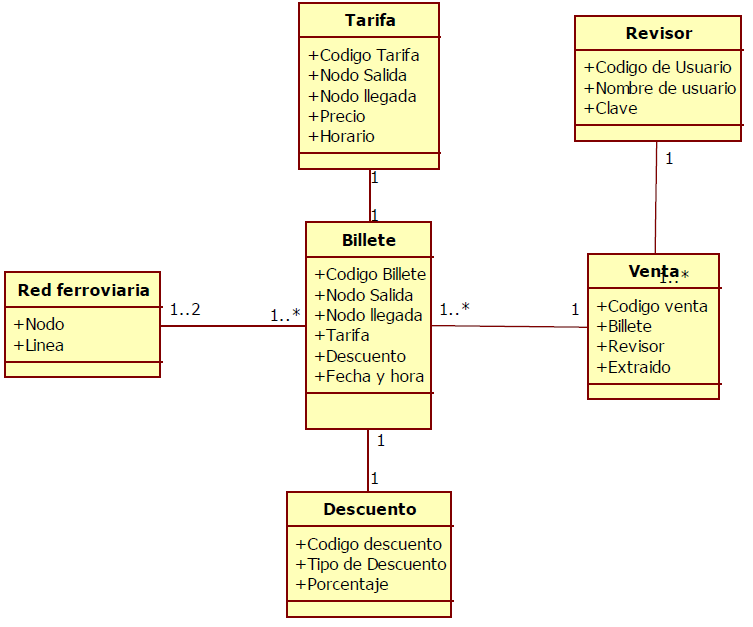
\includegraphics[width=0.7\linewidth]{./captura}
\label{fig:captura}
\end{figure}


Todos los datos serán alfanuméricos, sin embargo, el password deberá almacenarse de forma encriptada.\\

En términos de rendimiento, la base de datos debe alinearse con los requisitos de rendimiento de VIRUTA enunciados en la sección 3.3.\\

Dados los limitados recursos técnicos de los TPVs, la base de datos deberá ser lo más ligera posible.







\end{document}